\documentclass[12pt]{article}
\usepackage[margin=2.5cm]{geometry}
\usepackage{enumerate}
\usepackage{amsfonts}
\usepackage{amsmath}
\usepackage{fancyhdr}
\usepackage{amsmath}
\usepackage{amssymb}
\usepackage{amsthm}
\usepackage{mdframed}
\usepackage{graphicx}
\usepackage{subcaption}
\usepackage{adjustbox}
\usepackage{listings}
\usepackage{xcolor}
\usepackage{booktabs}
\usepackage[utf]{kotex}
\usepackage{hyperref}

\definecolor{codegreen}{rgb}{0,0.6,0}
\definecolor{codegray}{rgb}{0.5,0.5,0.5}
\definecolor{codepurple}{rgb}{0.58,0,0.82}
\definecolor{backcolour}{rgb}{0.95,0.95,0.92}

\lstdefinestyle{mystyle}{
    backgroundcolor=\color{backcolour},
    commentstyle=\color{codegreen},
    keywordstyle=\color{magenta},
    numberstyle=\tiny\color{codegray},
    stringstyle=\color{codepurple},
    basicstyle=\ttfamily\footnotesize,
    breakatwhitespace=false,
    breaklines=true,
    captionpos=b,
    keepspaces=true,
    numbers=left,
    numbersep=5pt,
    showspaces=false,
    showstringspaces=false,
    showtabs=false,
    tabsize=1
}

\lstset{style=mystyle}

\pagestyle{fancy}
\renewcommand{\headrulewidth}{0.4pt}
\lhead{CSC 209}
\rhead{Review 7 Solution}

\begin{document}
\title{CSC 209 Review 7 Solution}
\maketitle

\bigskip

\section{Exercises}

\begin{enumerate}[1.]
    \item

    First, I need to justify if the folllowing declarations legal on an individual basis:

    \bigskip

    \texttt{struct \{int x, y;\} x;}

    \texttt{struct \{int x, y;\} y;}

    \bigskip

    The struct \texttt{struct \{int x, y;\} x;} is legal. \texttt{struct \{int x, y;\} x;}
    is equivalent to

\begin{lstlisting}[language=c]
    struct {
            int x;
            int y;
    } x;
\end{lstlisting}

    and `x' beside struct represents variable of that type.

    \underline{\textbf{Notes}}

    \begin{itemize}
        \item \textbf{Declaring Structure Variables}

        \bigskip

        \begin{center}
        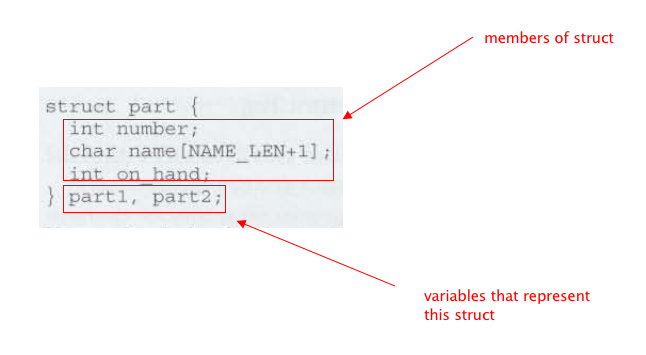
\includegraphics[width=\linewidth]{images/review_7_solution_1.png}
        \end{center}
    \end{itemize}
\end{enumerate}

\end{document}